\chapter{On the Practical uses of the Disintegrated Bounds}
\label{chap:dis-pra}
\addchapterlof
\addchapterloe

\vspace{-2.0cm}
\begin{center}
\textbf{This chapter is based on the following paper}\\[-0.1cm]
\end{center}
\printpublication{ViallardGermainHabrardMorvant2022}

\vspace{0.2cm}
\minitoc

\begin{abstract}
\vspace{-0.2cm}
PAC-Bayesian bounds are known to be tight and informative when studying the generalization ability of stochastic classifiers (see \eg, \Cref{chap:mv-sto}).
However, they require a loose and costly derandomization step when applied to some families of deterministic models such as neural networks.
As an alternative to this step, we introduce new PAC-Bayesian generalization bounds that have the originality to provide {\it disintegrated} bounds, \ie, they give guarantees over one {\it single} hypothesis instead of the usual {\it averaged} analysis.
Our bounds are easily optimizable and can be used to design self-bounding algorithms.
We illustrate this behavior on neural networks and show a significant practical improvement over the state-of-the-art framework.
\end{abstract}

\newpage
    
\section{Introduction}
\label{chap:dis-pra:sec:intro}

The PAC-Bayesian theory is a powerful framework for upper-bounding the true risk of stochastic models such as the stochastic majority vote (considered in \Cref{chap:mv-sto}).
Remember that, in general, the stochastic model samples an hypothesis from the posterior distribution and predicts a label with the sampled hypothesis.
However, the vast majority of machine learning methods nevertheless need guarantees on deterministic models (\ie that are not stochastic).
In this case, a {\it derandomization step} of the bound is required to get a bound on the deterministic model's risk.
In general, the {\it derandomization step} consists in obtaining a bound on the risk of a deterministic model from a bound originally valid for stochastic models.
Different forms of derandomization have been introduced in the literature for specific settings.
Among them, \citet{LangfordShaweTaylor2002} proposed a derandomization for Gaussian posteriors over linear classifiers: thanks to the Gaussian symmetry, a bound on the risk of the {\it maximum a posteriori} (deterministic) classifier is obtainable from the bound on the average risk of the stochastic classifier.
Also relying on Gaussian posteriors, \citet{LetarteGermainGuedjLaviolette2019} derived a PAC-Bayesian bound for a very specific deterministic network architecture using sign functions as activations; this approach has been further extended by \citet{BiggsGuedj2021,BiggsGuedj2022}.
Another line of works derandomizes neural networks~\citep{NeyshaburBhojanapalliSrebro2018, NagarajanKolter2019}.
While technically different, it starts from PAC-Bayesian guarantees on the stochastic classifier and uses an ``output perturbation'' bound to convert a guarantee from a random classifier to the mean classifier.
The relative diversity and specificity of these works highlight nevertheless the lack of a general framework for the derandomization of classic PAC-Bayesian bounds.\\

This chapter focuses on another kind of derandomization
through the {\it disintegration of the PAC-Bayesian bound}, proposed by \citet[Th.1.2.7]{Catoni2007} and \citet{BlanchardFleuret2007}; see \Cref{chap:pac-bayes:sec:disintegrated}.
Despite their interest in derandomizing PAC-Bayesian bounds, these kinds of bounds have only received little study in the literature and have never been used in practice.
Driven by machine learning practical purposes, our objective is thus twofold.
We derive new tight and usable {\it disintegrated} PAC-Bayesian bounds {\it (i)} that directly derandomize any classifiers without any other additional step and with {\it almost} no impact on the guarantee,  and {\it (ii)} that can be easily optimized to learn classifiers with strong guarantees.
To achieve this objective, our contribution consists in providing a new general disintegration framework based on the \textsc{Rényi} divergence (in \Cref{chap:dis-pra:theorem:disintegrated}), allowing us to meet the practical goal of efficient learning. 
From a theoretical standpoint, due to the \textsc{Rényi} divergence term, our bound is expected to be looser than the one of \citet[Th.1{\it(i)}]{RivasplataKuzborskijSzepesvariShaweTaylor2020} in which the divergence term is ``disintegrated'' but depends on the sampled hypothesis only.
However, as we show in our experimental evaluation on neural networks, their ``disintegrated'' term is, in practice, subject to high variance, making their bound harder to optimize. 
This variance arises because the sampled hypothesis does not influence our \textsc{Rényi} divergence term.
Our bound has then the main advantage of leading to a more stable learning algorithm  with better empirical results.
In addition, we derive in \Cref{chap:dis-pra:sec:info-theoretic} new theoretical results based on the mutual information, giving different insights into disintegration procedures.\\

The rest of the chapter is organized as follows.
\Cref{chap:dis-pra:sec:setting} recalled the notations we follow.
In \Cref{chap:dis-pra:sec:contrib}, we derive our main contribution relying on {\it disintegrated} PAC-Bayesian bounds.
Then, we illustrate the practical usefulness of this disintegration on deterministic neural networks in \Cref{chap:dis-pra:sec:expe}.
Before concluding in \Cref{chap:dis-pra:sec:conclu}, we discuss in \Cref{chap:dis-pra:sec:info-theoretic} another point of view of the disintegrated through an information-theoretic bound.
For readability, we deferred the proofs of our theoretical results to \Cref{ap:dis-pra}.

\section{Setting and PAC-Bayesian Bounds}
\label{chap:dis-pra:sec:setting}

In this chapter, we consider supervised classification tasks as described in \Cref{chap:pac-bayes} with $\X$ the input space, $\Y$ the label set, and $\D$ an unknown data distribution on $\X{\times}\Y$.
We consider a hypothesis set $\H$ of functions $\h:\X \to \Y$.
The learner aims to find  $\h\in\H$ that assigns a label $\y$ to an input $\x$ as accurately as possible. 
Given an example $(\x, \y)$ and a hypothesis $\h$, we assess the quality of the prediction of $\h$ with a loss function $\loss: \H\times (\X{\times}\Y) {\to} [0, 1]$ evaluating to which extent the prediction is accurate.
The learner wants to find the hypothesis $\h$ from $\H$ that minimizes the true risk $\RiskLoss_{\D}(\h)$. 
However, we cannot compute $\RiskLoss_{\D}(\h)=\EE_{(\x,\y)\sim\D}\loss(\h, (\x,\y))$ since the distribution $\D$ is unknown.
We only have access to a learning sample $\S=\{(\x_i,\y_i)\}_{i=1}^{\m}$ with the empirical risk defined as $\RiskLoss_{\dS}(\h)=\frac{1}{\m}\sum_{i=1}^{\m}\loss(\h, (\x_i,\y_i))$.\\

We now recall \citet{BeginGermainLavioletteRoy2016}'s general bound at the heart of our contribution (and introduced in \Cref{chap:pac-bayes:sec:pac-bayes}).
This bound depends on the \textsc{Rényi} divergence between $\Q$ and $\P$ defined as $\Renyi_{\lambda}(\Q\|\P) \defeq \frac{1}{\lambda{-}1}\ln\!\LB \text{\small${\displaystyle \EE_{\h{\sim}\P}}$}\!\LB\!\frac{ \Q(\h)}{\P(\h)}\RB^{\!\lambda}\RB$ with parameter $\lambda>1$.

\generalbegin*

A key notion here is that the PAC-Bayesian bounds apply on the expectation over the risk of the individual classifiers in $\H$; this randomization is the risk of the stochastic classifier.
A key issue for usual machine learning tasks is then the derandomization of the PAC-Bayesian bounds to obtain a guarantee for a deterministic classifier instead of a stochastic one (by removing the expectation on $\H$).
In some cases, this derandomization results from the structure of the hypotheses, such as for stochastic linear classifiers that can be directly expressed as one deterministic linear classifier~\citep{GermainLacasseLavioletteMarchand2009}.
However, in other cases, the derandomization is much more complex and specific to the class of hypotheses, such as for neural networks ({\it e.g.}, \citet{NeyshaburBhojanapalliSrebro2018}, \citet[Ap. J]{NagarajanKolter2019b}, \citet{BiggsGuedj2022}).\\

The next section states our main contribution to this chapter: a general derandomization framework based on the \textsc{Rényi} divergence for disintegrating PAC-Bayesian bounds into a bound for a single hypothesis from $\H$.

\section{Disintegrated PAC-Bayesian Theorems}
\label{chap:dis-pra:sec:contrib}

\subsection{Form of a Disintegrated PAC-Bayesian Bound}

We recall now the main form of a disintegrated PAC-Bayesian bound used in this chapter.

\definitiondesintegrated*

More precisely, the posterior $\AQ \defeq A(\S, \P)$ is defined through a given \textit{deterministic} algorithm $A:(\X{\times}\Y)^{\m}{\times}\M^{*}(\H) \to \M(\H)$ chosen \apriori.
The algorithm {\it (i)}~takes a learning sample  $\S\in(\X{\times}\Y)^{\m}$ and a prior distribution $\P\in\M^{*}(\H)$ as inputs, and {\it (ii)}~outputs a {\it data-dependent} distribution $\AQ\defeq A(\S, \P)$.
Concretely, this kind of generalization bound allows one to derandomize the usual PAC-Bayes bounds as follows.
Instead of considering a bound holding for all the posterior distributions on $\H$ as usually done in PAC-Bayes (the ``$\,\forall \Q\,$'' in \Cref{chap:pac-bayes:theorem:general-begin}), we consider only the posterior distribution $\AQ$ obtained through a deterministic algorithm $A$ taking the learning sample $\S$ and the prior $\P$ as inputs.
Then, the above bound holds for a unique hypothesis $\h{\sim}\AQ$ instead of the stochastic classifier: the individual risks are no longer averaged with respect to $\AQ$; this is the {\it PAC-Bayesian bound disintegration}.
The dependence in probability on $\AQ$ means that the bound is valid with probability at least $1{-}\delta$ over the random choice of the learning sample $\S{\sim}\D^\m$ and the hypothesis $\h{\sim}\AQ$.
Under this principle, we introduce in \Cref{chap:dis-pra:theorem:disintegrated,chap:dis-pra:theorem:disintegrated-lambda} below two new general disintegrated PAC-Bayesian bounds.
A key asset of our results is that the bounds are instantiable to specific settings  as for the ``classical'' PAC-Bayesian bounds (\eg, with \iid/non-\iid data, unbounded losses, etc.).
By instantiating such a bound, we obtain an easily optimizable bound, leading to a self-bounding algorithm~\citep{Freund1998} with theoretical guarantees.
As an illustration of the usefulness of our results, we provide, in \Cref{chap:dis-pra:sec:desintegration}, such an instantiation for neural networks.

\subsection{Disintegrated Bounds with the \textsc{Rényi} Divergence}

\subsubsection{Our Main Contribution: a General Disintegrated Bound}

In the same spirit as \Cref{chap:pac-bayes:theorem:general-begin} our main result stated in \Cref{chap:dis-pra:theorem:disintegrated} is a general bound involving the \textsc{Rényi} divergence $\Renyi_{\lambda}(\AQ\|\P)$ of order \mbox{$\lambda\!>\!1$}.
\begin{restatable}[General Disintegrated PAC-Bayes Bound]{theorem}{theoremdisintegrated}\label{chap:dis-pra:theorem:disintegrated} For any distribution $\D$ on $\X{\times}\Y$, for any hypothesis set $\H$, for any prior distribution $\P\in\M^{*}(\H)$, for any measurable function \mbox{$\varphi\!:\! \H{\times}(\X{\times}\Y)^{\m}{\to} \Rbb_{+}^*$}, for any \mbox{$\lambda\!>\!1$}, for any $\delta\in(0,1]$, for any algorithm \mbox{$A\!:\!(\X{\times}\Y)^{\m}{\times}\M^{*}(\H){\to} \M(\H)$}, we have
\begin{align*}
    \PP_{\S\sim\D^{\m},\h\sim \AQ}\!\Bigg(\! &\frac{\lambda}{\lambda{-}1}\ln\LP\varphi(\h,\!\S)\RP\\
    &\le  \ {\frac{2\lambda{-}1}{\lambda{-}1}}\ln\frac{2}{\delta}
 +\Renyi_{\lambda}(\AQ\|\P){+} \ln\LB\EE_{\S'{\sim}\D^{\m}}\EE_{\h'{\sim}\P}\LP\varphi(\h'\!, \S')^{\frac{\lambda}{\lambda{-}1}}\RP\RB \!\Bigg)\!\!\ge\! 1{-}\delta,
\end{align*}
\mbox{where $\AQ \defeq A(\S, \P)$ is output by the deterministic algorithm $A$}. 
\end{restatable}
\begin{noaddcontents}\begin{proof}[sketch (see \Cref{chap:dis-pra:sec:proof-disintegrated} for details)]
Recall that $\AQ$ is obtained 
with the algorithm $A(\S, \P)$.
Applying \textsc{Markov}'s inequality (\Cref{ap:tools:theorem:first-markov}) on $\varphi(\h,\!\S)$ with the random variable $\h$ and using \textsc{Hölder}'s inequality (\Cref{ap:tools:theorem:holder}) to introduce $\Renyi_{\lambda}(\AQ\|\P)$, we have,  with  probability at least $1{-}\tfrac\delta2$ on \mbox{$\S\!\sim\! \D^\m$ and $\h\!\sim\!\AQ$}, 
\begin{align*}
   \frac{\lambda}{\lambda{-}1}\ln\left[\varphi(\h,\!\S)\right] \ &\le\ \frac{\lambda}{\lambda{-}1}\ln\left[\frac{2}{\delta}\EE_{\h'{\sim} \AQ}\varphi(\h'\!, \S)\right]\\   
   &\le\  \Renyi_{\lambda}(\AQ\|\P)  + \frac{\lambda}{\lambda{-}1}\ln\frac{2}{\delta} +\ln\left[\EE_{\h'{\sim}\P}\LP\varphi(\h'\!, \S)^{\frac{\lambda}{\lambda-1}}\RP\right].
\end{align*}
By applying again \textsc{Markov}'s inequality (\Cref{ap:tools:theorem:first-markov}) on $\varphi(\h,\!\S)$ with the random variable $\S$, we have, with probability at least $1{-}\tfrac\delta2$ on \mbox{$\S\!\sim\! \D^\m$ and $\h\!\sim\!\AQ$},
\begin{align*}
\ln \left[\EE_{\h'{\sim}\P}
\LP\varphi(\h'\!, \S)^{\frac{\lambda}{\lambda{-}1}}\RP\right]
\le 
\ln\left[\frac{2}{\delta}\EE_{\S'{\sim}\D^{\m}}\EE_{\h'{\sim}\P}\LP\varphi(\h'\!, \S')^{\frac{\lambda}{\lambda{-}1}}\RP\right].
\end{align*}
Lastly, we combine the two bounds with a union bound argument.
\end{proof}\end{noaddcontents}

As for the general classical PAC-Bayesian bounds (\Cref{chap:pac-bayes:theorem:general-begin}), the above theorem can be seen as the starting point of the derivation of generalization bounds depending on the choice of the function~$\varphi$, as done in \Cref{chap:dis-pra:corollary:nn} in \Cref{chap:dis-pra:sec:training-method};
this property makes it the main result of this chapter. 
In its proof, \textsc{Hölder}'s inequality (\Cref{ap:tools:theorem:holder}) is used differently than in the classic PAC-Bayes bound's proofs.
Indeed, in the proof of \citet[Th. 8]{BeginGermainLavioletteRoy2016}, the change of measure based on \textsc{Hölder}'s inequality is key for deriving a bound that holds for all posteriors $\Q$ with high probability, while our bound holds for a unique \mbox{posterior $\AQ$} dependent on the sample $\S$ and the prior $\P$.
In fact, we use \textsc{Hölder}'s inequality to introduce a prior $\P$ independent from $\S$: a crucial point for our bound instantiated in \Cref{chap:dis-pra:corollary:nn}.
Compared to \Cref{chap:pac-bayes:theorem:general-begin}, our bound requires an additional term $\ln2{+}\frac{\lambda}{\lambda{-}1}\ln\tfrac{2}{\delta}$.
However, by setting  $\varphi(\h,\!\S)=m\,\kl(\RiskLoss_{\dS}(\h)\|\RiskLoss_{\D}(\h))$ and $\lambda{=}2$, 
the term $\ln\frac{8}{\delta^2}$ is multiplied by $\tfrac{1}{\m}$, which turns out to be a reasonable cost to ``derandomize'' a bound into a disintegrated one.
For instance, if $m=5,000$ (a reasonable sample size) and $\delta=0.05$, we have $\frac{1}{\m}\ln\tfrac{8}{\delta^2}\approx 0.002$.

We instantiate below \Cref{chap:dis-pra:theorem:disintegrated} for $\lambda{\rightarrow}1^+$ and $\lambda{\rightarrow}{+}{\infty}$ showing that the bound converges when $\lambda{\to}1^+$ and $\lambda{\to}{+}\infty$.
\begin{restatable}[Extreme Cases of \Cref{chap:dis-pra:theorem:disintegrated}]{corollary}{corollarydisintegrated}
Under the assumptions of  \Cref{chap:dis-pra:theorem:disintegrated}, when $\lambda{\to}1^+$,  we have
\begin{align*}
   \PP_{\S\sim\D^{\m},\h\sim \AQ}\!\Bigg(
  \ln\varphi(\h{,}\S) \le \ln\frac{2}{\delta} + \ln\left[\esssup_{\S'\in(\X{\times}\Y), \h'\in\H}\varphi(\h'{,} \S')\right]
  \Bigg)\!\ge\! 1{-}\delta,
\end{align*}
when $\lambda{\to}+\infty$,
we have
\begin{align*}
 \PP_{\S\sim\D^{\m},\h\sim \AQ}\!\Bigg(    \ln\varphi(\h{,} \S)\le\ln{\displaystyle\esssup_{\h'\in\H}}\,\frac{\AQ(\h')}{\P(\h')}{+}\ln\!\left[\frac{4}{\delta^2} {\displaystyle \EE_{\S'{\sim}\D^{\m}}\EE_{\h'{\sim}\P}\varphi(\h'{,}\S')}\right] \Bigg)\!\ge\! 1{-}\delta,
\end{align*}
where $\esssup$ is the essential supremum defined as the supremum on a set with non-zero probability measures, \ie, 
\begin{align*}
    &\esssup_{\S'\in(\X{\times}\Y), \h'\in\H}\varphi(\h'{,} \S')=\inf\LC\tau\in\Rbb, \PP_{\S\sim\D^{\m},\h\sim \AQ}\!\Big[ \varphi(\h{,} \S) > \tau\Big] = 0\RC,\\
    \text{and}\quad &\esssup_{\h'\in\H}\,\frac{\AQ(\h')}{\P(\h')}=\inf\LC\tau\in\Rbb, \PP_{\h\sim\AQ}\!\Big[ \tfrac{\AQ(\h)}{\P(\h)} > \tau\Big] = 0\RC.
\end{align*}
\label{chap:dis-pra:corollary:disintegrated}
\end{restatable}
\begin{noaddcontents}\begin{proof}
Deferred to~\Cref{chap:dis-pra:sec:proof-corollary-disintegrated}.
\end{proof}\end{noaddcontents}

This corollary illustrates that the parameter $\lambda$ controls the trade-off between the \textsc{Rényi} divergence 
$\Renyi_{\lambda}(\AQ\|\P)$ and 
$\ln\LB\EE_{\S'{\sim}\D^{\m}}\EE_{\h'{\sim}\P}\varphi(\h'\!, \S')^{\frac{\lambda}{\lambda{-}1}}\RB$. 
Indeed, when $\lambda{\rightarrow}1^+$, the \textsc{Rényi} divergence vanishes ($\Renyi_{\lambda}(\AQ\|\P){\to}0$) while the other term converges toward $\ln\!\left[\esssup_{\S'\in(\X{\times}\Y), \h'\in\H}\varphi(\h'\!, \S')\right]$, roughly speaking the maximal value possible for the second term.
On the other hand, when $\lambda{\rightarrow}{+}\infty$, the \textsc{Rényi} divergence increases and converges toward $\ln\esssup_{\h'\in\H}\frac{\AQ(\h')}{\P(\h')}$ and the other term decreases toward $\ln\!\left[\EE_{\S'{\sim}\D^{\m}}\EE_{\h'{\sim}\P}\varphi(\h'{,}\S')\right]$.

\subsubsection{Comparison with the Bound of~\citet{RivasplataKuzborskijSzepesvariShaweTaylor2020}}

For the sake of comparison, we recall in \Cref{chap:pac-bayes:theorem:general-disintegrated-rivasplata} the bound proposed by~\citet[Th.1{\it (i)}]{RivasplataKuzborskijSzepesvariShaweTaylor2020}, that is more general than the bounds of \citet{BlanchardFleuret2007} and \citet[Th.1.2.7]{Catoni2007}. 

\generaldisintegratedrivasplata*

Note that the bound can be rewritten with the logarithm, \ie, we have
\begin{align*}
\PP_{\S\sim\D^\m, \h\sim\AQ}\Bigg[ \ln\LP\varphi(\h,\S)\RP \le \ln\!\LB\frac{\AQ(\h)}{\P(\h)}\RB\!+\!\ln\!\LB\frac{1}{\delta}\EE_{\S'\sim\D^\m}\EE_{\h'\sim\P}
\varphi(\h',\S')\RB
\Bigg] \ge 1{-}\delta.    
\end{align*}
The term $\ln\!\tfrac{\AQ(\h)}{\P(\h)}$ (also involved in~\citet{Catoni2007,BlanchardFleuret2007}) can be seen as a ``disintegrated\footnote{We say that the KL divergence is ``disintegrated'' since the log term is not averaged in contrast to the KL divergence.} KL divergence'' depending only on the sampled  $\h{\sim}\AQ$.
In contrast, our bound involves the \textsc{Rényi} divergence $D_\lambda(\AQ\|\P)$ between the \mbox{prior $\P$} and the posterior $\AQ$, meaning our bound involves only one term that depends on the sample hypothesis (the risk): the divergence value is the same whatever the hypothesis.
Our bound is expected to be looser because of the \textsc{Rényi} divergence~\citep[see][]{ErvenHarremoes2014} and the dependence in $\delta$ (which is worse than in \Cref{chap:pac-bayes:theorem:general-disintegrated-rivasplata}).
Nevertheless, our divergence term is the main advantage of our bound.
Indeed, as confirmed by our experiments (\Cref{chap:dis-pra:sec:expe}), our bound with $\Renyi_{\lambda}(\AQ\|\P)$ makes the learning procedure (in our self-bounding algorithm) more stable and efficient compared to the optimization of \Cref{chap:pac-bayes:theorem:general-disintegrated-rivasplata}'s bound with $\ln\tfrac{\AQ(\h)}{\P(\h)}$ that is subject to high variance.
  
\subsubsection{A Parameterizable General Disintegrated  Bound}

In the PAC-Bayesian literature, parameterized bounds have been introduced ({\it e.g.}, \citet{Catoni2007, ThiemannIgelWintenbergerSeldin2017}) to control the trade-off  between the empirical risk and the divergence along with the additional term. 
For the sake of completeness, we now provide a parameterized version of our bound, enlarging its practical scope.
 We follow a similar approach to introduce a version of a disintegrated \textsc{Rényi} divergence-based bound that has the advantage of being parameterizable.
\begin{restatable}[Parametrizable Disintegrated PAC-Bayes Bound]{theorem}{theoremdisintegratedlambda} For any distribution $\D$ on $\X{\times}\Y$, for any hypothesis set $\H$, for any prior distribution $\P\in\M^{*}(\H)$, for any measurable function \mbox{$\varphi\!:\! \H{\times}(\X{\times}\Y)^{\m}{\to} \Rbb_{+}^*$}, for any $\delta\in(0,1]$, for any algorithm \mbox{$A\!:\!(\X{\times}\Y)^{\m}{\times}\M^{*}(\H){\to} \M(\H)$}, we have
\begin{align*}
&\PP_{\substack{\S\sim\D^{\m},\\\h\sim \AQ}} \!\Bigg(\!\forall\lambda{>}0,\,\ln\LP\varphi(\h,\!\S)\RP{\le} \ln\!\bigg[
\frac\lambda 2\displaystyle e^{\Renyi_{2}(\AQ\|\P)}{+} \frac{8}{2\lambda\delta^3}\EE_{\S'{\sim}\D^{\m}}\EE_{\h'{\sim}\P}\!\Big[\varphi(\h'\!, \S')^2\Big]
\bigg]\!\Bigg)\ge1{-}\delta,
\end{align*}
\mbox{where $\AQ{\defeq}A(\S,\P)$ is output by the deterministic algorithm $A$}. 
\label{chap:dis-pra:theorem:disintegrated-lambda} 
\end{restatable}
\begin{noaddcontents}\begin{proof}
Deferred to~\Cref{chap:dis-pra:sec:proof-disintegrated-lambda}.
\end{proof}\end{noaddcontents}

Note that $e^{\Renyi_{2}(\AQ\|\P)}$ is closely related to the $\chi^2$-distance. Indeed we have: $\chi^2(\AQ\|\P) \defeq \EE_{\h\sim\P}\LB\tfrac{\AQ(\h)}{\P(\h)}\RB^2\!\!{-}1 = e^{\Renyi_{2}(\AQ\|\P)} {-}1$.
An asset of \Cref{chap:dis-pra:theorem:disintegrated-lambda} is the parameter $\lambda$ controlling the trade-off between the exponentiated \textsc{Rényi} divergence $e^{\Renyi_{2}(\AQ\|\P)}$ and $\frac{1}{\delta^3}{\EE}_{\S'{\sim}\D^{\m}}{\EE}_{\h'{\sim}\P}\varphi(\h'\!, \S')^2$.
Our bound is valid for all \mbox{$\lambda\!>\!0$}, thus, from a practical view, we can learn/tune the parameter $\lambda$ to minimize the bound and control the possible numerical instability due to  $e^{\Renyi_{2}(\AQ\|\P)}$.
Indeed, if $\Renyi_{2}(\AQ\|\P)$ is large, the numerical computation can lead to an infinite value due to finite precision arithmetic.
It is important to notice that, like other parameterized bounds \citep[\eg,][]{ThiemannIgelWintenbergerSeldin2017}, there exists a closed-form solution of the optimal parameter $\lambda$ (for a fixed $\P$ and $ \AQ$); the solution is derived in \Cref{chap:dis-pra:prop:lambda-min} and shows that the optimal bound of \Cref{chap:dis-pra:theorem:disintegrated-lambda} corresponds to the bound of \Cref{chap:dis-pra:theorem:disintegrated}.

\begin{restatable}[Optimal Bound of \Cref{chap:dis-pra:theorem:disintegrated-lambda}]{proposition}{proplambdamin}\label{chap:dis-pra:prop:lambda-min} For any distribution $\D$ on $\X{\times}\Y$, for any hypothesis set $\H$, for any prior distribution $\P$ on $\H$, for any $\delta{\in}(0,1]$, for any measurable function $\varphi\!:\! \H{\times}(\X{\times}\Y)^{\m}{\to} \Rbb_{+}^*$, for any algorithm $A\!:\!(\X{\times}\Y)^{\m}{\times}\M^{*}(\H){\to} \M(\H)$, let 
\begin{align*}
\lambda^* {=} \argmin_{\lambda>0} \, \ln\! \left[\frac{\lambda}{2} e^{\Renyi_{2}(\AQ\|\P)}\!+\!
\frac{\displaystyle \EE_{{\S'{\sim}\D^{\m}}} \EE_{\h'{\sim}\P}\,\LB8\varphi(\h'\!, \S')^2\RB}{2\lambda\delta^3}  \right]\!,
\end{align*}
\begin{align*}
\mbox{then, we have}\quad & \overbrace{2\ln\!\LB\frac{\lambda^*}{2\ }e^{\Renyi_{2}(\AQ\|\P)}\!+\! \EE_{\S'{\sim}\D^{\m}}\EE_{\h'{\sim} \P}
\LP\frac{8\varphi(\h'\!, \S')^2}{2\lambda^*\delta^3}\RP\RB}^{\text{\Cref{chap:dis-pra:theorem:disintegrated-lambda}}}   \\ &= \ \underbrace{\Renyi_{2}(\AQ\|\P) + \ln\LB\EE_{\S'{\sim}\D^{\m}}\EE_{\h'{\sim} \P}
\LP\frac{8\varphi(\h'\!, \S')^{2}}{\delta^3}\RP\RB}_{\text{\Cref{chap:dis-pra:theorem:disintegrated} with $\lambda=2$.} },
\end{align*}
where  $\displaystyle \lambda^* = \sqrt{\frac{\EE_{\S'{\sim}\D^{\m}}{\EE}_{{\h'{\sim}\P}}\LB8\varphi(\h'\!, \S')^2\RB}{\delta^3 \exp(\Renyi_{2}(\AQ\|\P))}}$. \\[1mm]
Put into words: the optimal $\lambda^*$ gives the same bound for \Cref{chap:dis-pra:theorem:disintegrated} and \Cref{chap:dis-pra:theorem:disintegrated-lambda}.
\end{restatable}
\begin{noaddcontents}\begin{proof}
Deferred to~\Cref{chap:dis-pra:sec:proof-min-lambda}.
\end{proof}\end{noaddcontents}

\section{The Disintegration in Action}
\label{chap:dis-pra:sec:desintegration}

So far, we have introduced theoretical results to derandomize PAC-Bayesian bounds through a disintegration approach.
Indeed, the disintegration allows us to obtain a bound for a unique model sampled from $\AQ$ instead of having a bound on the averaged risk.
This section proposes to illustrate the instantiation and usefulness of \Cref{chap:dis-pra:theorem:disintegrated} on neural networks compared to the classical PAC-Bayesian bounds.

\subsection{Specialization to Neural Network Classifiers}
\label{chap:dis-pra:sec:training-method}

We aim to learn the weights of the Neural Networks (NN) leading to the lowest true risk $\Risk_{\D}(\h)=\EE_{(\x,\y)\sim\D}\indic\LB \h(\x)\ne \y\RB$.
In other words, we consider that the hypothesis set $\H$ is a set of neural networks with different weights for a given architecture.
Practitioners usually proceed by epochs and obtain one ``intermediate''  NN after each epoch.
Then, they select the ``intermediate''  NN associated with the lowest validation risk.
We propose translating this practice into our PAC-Bayesian setting by considering one prior per epoch.
Given $\iter$ epochs, we hence have
$\iter$ priors $\priorset{=}\{\P_\t\}_{\t=1}^\iter$, where \mbox{$\forall \t\!\in\!\{1,\ldots,\iter\}, \P_\t=\Ncal(\vbf_\t, \sigma^2\Ibf_{D})$} is a Gaussian distribution centered \mbox{at $\vbf_\t$} (the weight vector associated with the \mbox{$\t$-th} ``intermediate''  NN) with a covariance matrix of $\sigma^2\Ibf_{D}$ (where $\Ibf_{D}$ is the $D{\times}D$-dimensional identity matrix).
Assuming the $\iter$ priors are learned from a set $\S_{\text{prior}}$ such that \mbox{$\S_{\text{prior}} \bigcap \S {=} \emptyset$}, then 
\Cref{chap:dis-pra:corollary:nn,chap:dis-pra:corollary:nn-rbc} will guide us to learn a posterior \mbox{$\AQ{=}\Ncal(\wbf, \sigma^2\Ibf_{D})$} from the prior $\P\in\priorset$ minimizing the empirical risk on $\S$ (we give more details on the procedure after the forthcoming corollaries).
Note that considering Gaussian distributions has the advantage of simplifying the expression of the KL divergence and thus is commonly used in the PAC-Bayesian literature for neural networks \citep[\eg, ][]{DziugaiteRoy2017,LetarteGermainGuedjLaviolette2019,ZhouVeitchAusternAdamsOrbanz2019}.\footnote{This has been first studied in  the context of linear classifiers \citep[\eg, ][]{AmbroladzeHernandezTaylor2006,GermainLacasseLavioletteMarchand2009,GermainHabrardLavioletteMorvant2020}.
However, in this context the symmetry of the Gaussian distribution also ease the derandomization.}

\Cref{chap:dis-pra:corollary:nn} below instantiates \Cref{chap:dis-pra:theorem:disintegrated} to this neural networks setting.
Then, for the sake of comparison, \Cref{chap:dis-pra:corollary:nn-rbc} instantiates other disintegrated bounds from the literature; more precisely, \Cref{chap:dis-pra:eq:nn-rivasplata} corresponds to \citet{RivasplataKuzborskijSzepesvariShaweTaylor2020}'s bound of \Cref{chap:pac-bayes:theorem:general-disintegrated-rivasplata}, \Cref{chap:dis-pra:eq:nn-blanchard} to \citet{BlanchardFleuret2007}'s one,  and \Cref{chap:dis-pra:eq:nn-catoni} to \citet{Catoni2007}'s one.

\begin{restatable}[Instantiation of \Cref{chap:dis-pra:theorem:disintegrated} for Neural Networks]{corollary}{corollarynn}\label{chap:dis-pra:corollary:nn} For any distribution $\D$ on $\X{\times}\Y$, for any set \mbox{$\priorset=\{\P_1,\dots, \P_\iter\}$} of $\iter$ priors on $\H$ where $\P_\t=\Ncal(\vbf_\t, \sigma^2\Ibf_D)$, for any algorithm $A\!:\!(\X{\times}\Y)^{\m}\times\M^{*}(\H) {\rightarrow} \M(\H)$, for any loss $\ell\!:\! \H{\times} (\X{\times}\Y) {\to} [0, 1]$, for any $\delta{\in}(0,1]$,
we have 
\begin{align*}
 \PP_{\S\sim\D^{\m}, \h\sim \AQ}\Bigg(\forall& \P_\t\in \priorset,\ \kl(\RiskLoss_{\dS}(\h)\| \RiskLoss_{\D}(\h))\le \frac{1}{\m}\left[ \frac{\|\wbf{-}\vbf_\t\|_{2}^{2}}{\sigma^2}+\ln\frac{16\iter\sqrt{\m}}{\delta^3}\right]\!\Bigg)\geq 1{-}\delta,
\end{align*}
where $\kl(a\|b) = a\ln\tfrac{a}{b}+(1{-}a)\ln\tfrac{1-a}{1-b}$, $\AQ = \Ncal(\wbf, \sigma^2\Ibf_D)$, and the hypothesis $\h\sim\AQ$ is parameterized by $\wbf{+}\epsilonbf$.
\end{restatable}
\begin{noaddcontents}\begin{proof}
Deferred to~\Cref{chap:dis-pra:sec:proof-corollary-nn}.
\end{proof}\end{noaddcontents}

\begin{restatable}[Instantiation of Known Bounds for Neural Networks]{corollary}{corollarynnrbc}\label{chap:dis-pra:corollary:nn-rbc} For any distribution $\D$ on $\X{\times}\Y$, for any set \mbox{$\priorset=\{\P_1,\dots,\P_\iter\}$} of $\iter$ priors on $\H$ where $\P_\t=\Ncal(\vbf_\t, \sigma^2\Ibf_D)$, for any algorithm $A\!:\!(\X{\times}\Y)^{\m}\times\M^{*}(\H){\rightarrow} \M(\H)$, for any loss $\ell\!:\! \H{\times} (\X{\times}\Y) {\to} \{0, 1\}$, for any $\delta{\in}(0,1]$,  with probability at least $1{-}\delta$ over the learning sample $\S{\sim}\D^{\m}$ and the hypothesis $\h{\sim} \AQ$ parameterized by $\wbf{+}\epsilonbf$, we have $\forall \P_\t\in \priorset$
\begin{align}
&\kl(\RiskLoss_{\dS}(\h)\|\RiskLoss_{\D}(\h))\!\le\, \frac{1}{\m}\! \Bigg[\! 
\frac{\| \wbf{+}\epsilonbf{-}\vbf_\t\|^2_{2} {-}\|\epsilonbf\|^2_{2}}{2\sigma^2} {+}  \ln\! \frac{2\iter\!\sqrt{\m}}{\delta}\!\Bigg]\!,\!\label{chap:dis-pra:eq:nn-rivasplata} \\
\forall b\!\in\!\blaset, &\kl_{+}(\RiskLoss_{\dS}(\h)\|\RiskLoss_{\D}(\h))\!\le \frac{1}{\m} \! \Bigg[
\frac{b{+}1}{b}\!\LB\frac{\| \wbf{+}\epsilonbf{-}\vbf_\t\|^2_{2} {-}\|\epsilonbf\|^2_{2}}{2\sigma^2}\RB_{\!+}\!\!\!\!{+}  \ln\! \frac{(b{+}1)\iter\card(\blaset)}{\delta} \Bigg]\!,\!\label{chap:dis-pra:eq:nn-blanchard}\\
\forall c\!\in\!\catset,\ &\RiskLoss_{\D}(\h) \!\le \frac{\displaystyle1{-}\exp\!\left({\displaystyle\!\!{-}c\RiskLoss_{\dS}(\h) {-}\frac{1}{\m}\!\!\left[\! \frac{\| \wbf{+}\epsilonbf{-}\vbf_\t\|^2_{2} {-}\|\epsilonbf\|^2_{2}}{2\sigma^2} {+} \ln\!\frac{\iter\card(\catset)}{\delta}\!\right]\!}\right)}{1{-}e^{{-}c}},\label{chap:dis-pra:eq:nn-catoni}
\end{align}
with $\LB x\RB_{+}\!{=}\max(x,0)$, and   $\kl_{+}(\RiskLoss_{\dS}(\h)\|\RiskLoss_{\D}(\h)){=}\kl(\RiskLoss_{\dS}(\h)\|\RiskLoss_{\D}(\h))$ if $\RiskLoss_{\dS}(\h){<}\RiskLoss_{\D}(\h)$ and 0 otherwise.
Moreover, $\epsilonbf{\sim}\Ncal(\zerobf, \sigma^2\Ibf_{D})$ is a Gaussian noise such that $\wbf{+}\epsilonbf$ are the weights of $\h{\sim}\AQ$ with \mbox{$\AQ{=}\Ncal(\wbf, \sigma^2\Ibf_{D})$}, and $\catset$, $\blaset$ are two sets of hyperparameters fixed a priori.
\end{restatable}
\begin{noaddcontents}\begin{proof}
Deferred to~\Cref{chap:dis-pra:sec:proof-corollary-nn-rbc}.
\end{proof}\end{noaddcontents}

Since we aim to minimize the true risk $\Risk_{\D}(\h)$, \ie, we consider in practice the 01-loss $\loss(\h,(\x,\y))=\indic\LB\h(\x)\ne \y\RB$.
As the parameter $\lambda$ of the \Cref{chap:dis-pra:theorem:disintegrated-lambda}, $c\!\in\!\catset$ is a hyperparameter that controls a trade-off between the empirical risk $\RiskLoss_{\dS}(\h)$ and $\frac{1}{\m}\!\!\left[\! \frac{\| \wbf{+}\epsilonbf{-}\vbf_\t\|^2_{2} {-}\|\epsilonbf\|^2_{2}}{2\sigma^2} {+} \ln\!\frac{\iter\card(\catset)}{\delta}\!\right]$.
Besides, the parameter $b\!\in\!\blaset$ controls the tightness of the bound. 
These parameters can generally be tuned to minimize the bound of \Cref{chap:dis-pra:eq:nn-blanchard} and \Cref{chap:dis-pra:eq:nn-catoni}; however, there is no closed-form solution for the expression of the minimum of these equations.
Consequently, our experimental protocol requires minimizing the bounds by gradient descent for each $b\!\in\!\blaset$ or $c\!\in\!\catset$ to learn the distribution $\AQ$ leading to the lowest bound value.
To obtain a tight bound, the divergence between one prior $\P_\t\!\in\!\priorset$ and $ \AQ$ must be low, \ie,  $\| \wbf{-}\vbf_\t\|_{2}^2$ (or $\| \wbf{+}\epsilonbf{-}\vbf_\t\|_{2}^2{-}\|\epsilonbf\|^2_{2}$) has to be small.
One solution 
is to split the learning sample into $2$ non-overlapping subsets  $\S_{\text{prior}}$ and $\S$, where $\S_{\text{prior}}$ is used to learn the prior, while $\S$ is used both to learn the posterior and compute the bound.
Hence, if we ``pre-learn'' a good enough prior $\P_\t\!\in\!\priorset$ from $\S_{\text{prior}}$, then we can expect to have a low \mbox{$\| \wbf{-}\vbf_\t\|_{2}$}.

\begin{minipage}{1.0\linewidth}
\begin{training}{\bf Training Method}
The original training set is split in two distinct subsets: $\S_{\text{prior}}$  and $\S$ (respectively of size $\m_{\text{prior}}$ and $\m$, that can be different).\\
The training has two phases.\\
{\bf 1)} The prior distribution $\P$ is ``pre-learned'' with $\S_{\text{prior}}$ and selected by early stopping,  with $\S$ as validation set, using the algorithm $A_{\text{prior}}$ (an arbitrary learning algorithm).\\
{\bf 2)} Given $\S$ and $\P$, we learn the posterior $\AQ$ with the algorithm $A$ (defined {\it a priori}).
\end{training}
\end{minipage}\\

\looseness=-1
At first sight, the selection of the prior weights with $\S$ by early stopping may appear to be ``cheating''.
However, this procedure can be seen as: {\it (i)}~first constructing $\priorset$ from the $\iter$ ``intermediate'' NNs learned after each epoch \mbox{from $\S_{\text{prior}}$}, then  {\it (ii)}~optimizing the bound with the prior that leads to the best risk \mbox{on $\S$}.
This gives a statistically valid result: since \Cref{chap:dis-pra:corollary:nn} is valid for every $\P_\t\!\in\!\priorset$, we can select the one we want, in particular the one minimizing  $\RiskLoss_{\dS}(\h)$ for a sampled $\h\sim\P_\t$.
This heuristic makes sense: it allows us to detect if a prior is concentrated around hypotheses that potentially overfit the learning sample $\S_{\text{prior}}$.
Usually, practitioners consider this ``best'' prior as the final  NN.
In our case, the advantage is that  we refine this ``best'' prior with $\S$ to learn the posterior $ \AQ$.
Note that \citet{PerezOrtizRivasplataShaweTaylorSzepesvari2021} have already  introduced tight generalization bounds with data-dependent priors for---non-derandomized---stochastic  NNs.
Nevertheless, our training method to learn the prior differs greatly since {\it (i)}~we learn $\iter$  NNs (\ie, $\iter$ priors) instead of only one, {\it (ii)}~we fix the variance of the Gaussian in the posterior  $\AQ$.
To the best of our knowledge, our training method for the prior is new.


\subsection{A Note About Stochastic Neural Networks}
Due to its stochastic nature, PAC-Bayesian theory has been explored to study stochastic  NNs (\eg,~\citet{DziugaiteRoy2017, DziugaiteRoy2018, ZhouVeitchAusternAdamsOrbanz2019, PerezOrtizRivasplataShaweTaylorSzepesvari2021}).
In \Cref{chap:dis-pra:corollary:nn-sto} below, we instantiate the bound of \Cref{chap:pac-bayes:theorem:general-germain} for stochastic  NNs to empirically compare the stochastic and the deterministic  NNs associated with the same prior and posterior distributions.
We recall that, in this chapter, a deterministic  NN is a \emph{single} $\h$ sampled from the posterior distribution $\AQ{=}\Ncal(\wbf, \sigma^2\Ibf_{D})$ output by the algorithm $A$.
Hence, for each example, the prediction is performed by the same deterministic NN: the one parameterized by the weights $\wbf+\epsilonbf\!\in\! \R^D$.
Conversely, the stochastic  NN associated with a posterior distribution $\Q{=}\Ncal(\wbf, \sigma^2\Ibf_{D})$ predicts the label of a given example by {\it(i)} first sampling $\h$ according to $\Q$, and {\it (ii)} then returning the label predicted \mbox{by $\h$.}
Thus, the risk of the stochastic  NN is the expected risk value $\EE_{\h{\sim}\Q}\RiskLoss_{\D}(\h)$, where the expectation is taken over \mbox{\emph{all} $\h$ sampled from $\Q$}.
We compute the empirical risk of the stochastic  NN from a Monte Carlo approximation:  {\it (i)} we sample $\K$ weight vectors, and {\it (ii)} we average the risk over the $\K$ associated NNs;
we denote by $\Q^\K$ the distribution of such $\K$-sample.
In this context, we obtain the following PAC-Bayesian bound.

\begin{restatable}[PAC-Bayesian Bound for Stochastic Neural Networks]{corollary}{corollarynnsto}\label{chap:dis-pra:corollary:nn-sto}
For any distribution $\D$ on $\X{\times}\Y$, for any set $\priorset=\{\P_1,\dots, \P_\iter\}$ of $\iter$ priors on $\H$ where $\P_\t=\Ncal(\vbf_\t, \sigma^2\Ibf_D)$, for any loss $\ell\!:\! \H{\times} (\X{\times}\Y) {\to} \{0, 1\}$, for any $\delta{\in}(0,1]$, with probability at least $1{-}\delta$ over $\S{\sim}\D^\m$ and $\{h_1,\dots,h_\K\}{\sim}\Q^\K$, we have simultaneously $\forall \P_\t\!\in\!\priorset,$
\begin{align}
&\kl\!\left(\EE_{\h{\sim}\Q}\!\!\RiskLoss_{\dS}(\h)\|\! \EE_{\h{\sim}\Q}\!\!\RiskLoss_{\D}(\h)\!\right)\!
{\le} \frac{1}{\m}\!\!\LB 
\frac{\|\wbf\!{-}\vbf_\t\|_{2}^{2}}{2\sigma^2}
{+}\ln\!\frac{4\iter\sqrt{\m}}{\delta}\RB\!,\!\label{chap:dis-pra:eq:nn-sto-seeger}\\
\!\!\mbox{and }\quad  &\kl\LP{\frac{1}{\K}\sum_{i=1}^{\K}\!\Risk_{\S}(\h_i)}\|\EE_{\h{\sim}\Q}\!\RiskLoss_{\dS}(\h)\RP \le \frac1n \ln\frac{4}{\delta}, \label{chap:dis-pra:eq:nn-sto-sample}
\end{align}
where $\Q=\Ncal(\wbf, \sigma^2\Ibf_D)$ and the hypothesis $\h$ sampled from $\Q$ is parameterized by $\wbf+\epsilonbf$ with $\epsilonbf\sim\Ncal(\zerobf, \sigma^2\Ibf_D)$.
\end{restatable}
\begin{noaddcontents}\begin{proof}
Deferred to~\Cref{chap:dis-pra:sec:proof-nn-sto}.
\end{proof}\end{noaddcontents}

\looseness=-1
This result shows two features that allow considering it as an adapted baseline for a fair comparison 
between disintegrated and classical PAC-Bayesian bounds,  thus between deterministic and stochastic NNs.
Firstly, it involves the same terms as \Cref{chap:dis-pra:corollary:nn}.
Secondly, it is close to the bound of~\citet[Sec.~6.2]{PerezOrtizRivasplataShaweTaylorSzepesvari2021}, since {\it (i)} we adapt the KL divergence to our setting (\ie, $\KL(\Q\|\P){=}\tfrac{1}{2\sigma^2}\|\wbf{-}\vbf_\t\|_2^2$), {\it (ii)} the bound holds for $\iter$ priors thanks to a union bound argument.

\section{Experiments with Neural Networks}
\label{chap:dis-pra:sec:expe}

In this section, we do not seek state-of-the-art performance; in fact, we have a threefold objective:
{\it (i)} we check if $50\%/50\%$ is a good choice for splitting the original train set into $(\S_{\text{prior}}, \S)$ (which is the most common split in the PAC-Bayesian literature~\citep{GermainLacasseLavioletteMarchand2009,PerezOrtizRivasplataShaweTaylorSzepesvari2021});
{\it (ii)} we highlight that our disintegrated bound associated with the deterministic NN is tighter than the randomized bound associated with the stochastic NN (\Cref{chap:dis-pra:corollary:nn-sto});
{\it (iii)} we show that our disintegrated bound (\Cref{chap:dis-pra:corollary:nn}) is tighter and more stable than the ones based on \citet{RivasplataKuzborskijSzepesvariShaweTaylor2020}, \citet{BlanchardFleuret2007} and \citet{Catoni2007} (\Cref{chap:dis-pra:corollary:nn-rbc}).

\subsection{Training Method}
We follow our Training Method (\Cref{chap:dis-pra:sec:training-method}) in which we integrate the direct minimization of all the bounds.
We refer as \algoours the training method based on the minimization of our bound in \Cref{chap:dis-pra:corollary:nn}, as \algorivasplata the one based on \Cref{chap:dis-pra:eq:nn-rivasplata}, as \algoblanchard the one based on \Cref{chap:dis-pra:eq:nn-blanchard}, and as \algocatoni the one based on \Cref{chap:dis-pra:eq:nn-catoni}.
\algostoNN denotes the PAC-Bayesian bound with the prior and posterior distributions obtained from \algoours.
To optimize the bound with gradient descent, we replace the non-differentiable 0-1 loss $\indic\LB \h(\x)\ne\y\RB$ with a surrogate: the bounded cross-entropy loss \citep{DziugaiteRoy2018}.
We made this replacement since cross-entropy minimization works well in practice for neural networks \citep{GoodfellowBengioCourville2016} and because this loss is bounded between 0 and 1, which is required for the $\kl()$ function.
The cross-entropy is defined in a multi-class setting with \mbox{$\y\in\Y$} by \mbox{$\loss(\h, (\x,\y)) = -\frac{1}{Z}\ln\!\LB e^{-Z}+(1-2e^{-Z})\h[y]\RB \in [0, 1]$} where $\h[y]$ is the \mbox{$\y$-th} output of the  NN; we set $Z{=}4$, the default parameter of \citet{DziugaiteRoy2018}.
That being said, to learn a good enough prior $\P\!\in\!\priorset$ and the posterior $\AQ$, we run our Training Method with two stochastic gradient descent-based algorithms $A_{\text{prior}}$ and $A$.
Note that the randomness in the stochastic gradient descent algorithm is fixed to have deterministic algorithms.
In phase {\bf 1)} algorithm $A_{\text{prior}}$ learns from $\S_{\text{prior}}$  the $\iter$ priors \mbox{$\P_1,\dots,\P_\iter\!\in\!\priorset$} (\ie, during $\iter$ epochs)  by minimizing the bounded cross-entropy loss.
In other words, at the end of the epoch $\t$, the weights $\wbf_\t$ of the classifier are used to define the prior $\P_\t=\Ncal(\wbf_\t, \sigma^2\Ibf_{D})$.
Then, the best prior $\P\!\in\!\priorset$ is selected by early stopping on $\S$.
In phase {\bf 2)}, given $\S$ and $\P$, 
algorithm $A$ integrates the direct optimization of the bounds with the bounded cross-entropy loss.
\subsection[Optimization Procedure in Algorithms $A$ and $A_{\text{prior}}$]{Optimization\protect\footnote{The details of the optimization and the evaluation of the bounds are described in Appendix.} Procedure in Algorithms $A$ and $A_{\text{prior}}$}
Let $\omegabf$ be the mean vector of a Gaussian distribution used as NN weights that we are optimizing.
In algorithms $A$ and $A_{\text{prior}}$, we use the Adam optimizer ~\citep{KingmaBa2015}, and we sample a noise ${\epsilonbf}\!\sim\! \Ncal({\bf 0}, \sigma^2\Ibf_{D})$ at each iteration of the optimizer.
Then, we forward the examples of the mini-batch in the NN parameterized by the weights $\omegabf{+}\epsilonbf$, and we update $\omegabf$ according to the bounded cross-entropy loss. 
Note that during phase {\bf 1)}, at the end of each epoch $\t$, $\P_{\t} {=} \Ncal(\omegabf, \sigma^2\Ibf_{D}) {=} \Ncal(\vbf_\t, \sigma^2\Ibf_{D})$ and finally at the end of phase {\bf 2)} we have $\AQ {=} \Ncal(\omegabf, \sigma^2\Ibf_{D}) {=} \Ncal(\wbf, \sigma^2\Ibf_{D})$.

\subsection{Experimental Setting}

\subsubsection{Datasets}
We perform our experimental study on three datasets: MNIST~\citep{LeCunCortesBurges1998},  Fashion-MNIST~\citep{XiaoRasulVollgraf2017}, and  CIFAR-10~\citep{Krizhevsky2009}. 
We divide each original train set into two independent subsets $\S_{\text{prior}}$ of size $\m_{\text{prior}}$ and $\S$ of size $\m$ with varying split ratios defined as $\tfrac{\m_{\text{prior}}}{\m+\m_{\text{prior}}}\in\{0, .1, .2, .3, .4, .5, .6, .7, .8, .9\}$.
The test sets denoted by $\T$ remain the original ones.

\subsubsection{Models}
\label{chap:dis-pra:sec:models}

\looseness=-1
For the (Fashion-)MNIST datasets, we train a variant of the All Convolutional  Network~\citep{SpringenbergDosovitskiyBroxRiedmiller2014}.
The model is a $3$-hidden layers convolutional network with $96$ channels.
We use $5\times 5$ convolutions  with a padding of size $1$ and a stride of size 1 everywhere except on the second convolution where we use a stride of size $2$.
We adopt the Leaky ReLU activation functions after each convolution. Lastly, we use a global average pooling of size $8\times 8$ to obtain the desired output size. 
Furthermore, the weights are initialized with Xavier Normal initializer~\citep{GlorotBengio2010} while each bias of size $l$ is initialized uniformly between $-1/{\sqrt{l}}$ and $1/\sqrt{l}$.
For the CIFAR-10 dataset, we train a ResNet-20 network, \ie, a ResNet network from \citet{HeZhangRenSun2016} with $20$ layers.
The weights are initialized with Kaiming Normal initializer~\citep{HeZhangRenSun2015} and each bias of size $l$ is initialized uniformly between $-1/{\sqrt{l}}$ and $1/\sqrt{l}$.


\subsubsection{Optimization}

\looseness=-1
For the (Fashion-)MNIST datasets, we learn the parameters of our prior distributions $\P_1,\dots,\P_\iter$ by using Adam optimizer for $\iter=10$ epochs with a learning rate of $\lr=10^{-3}$ and a batch size of $32$ (the other parameters of Adam are left by default).
Moreover, the posterior distribution's parameters are learned for one epoch with the same batch size and optimizer (except that the learning rate is either $\lr=10^{-4}$ or $\lr=10^{-6}$).
For the CIFAR-10 dataset, the parameters of the priors $\P_1,\dots,\P_\iter$ are learned for $\iter=100$ epochs and the posterior distribution $\AQ$ for $10$ epochs with a batch size of $32$ by using Adam optimizer as well. 
Additionally, the learning rate to learn the prior for CIFAR-10 is $\lr=10^{-2}$.

\subsubsection{Bounds}

\looseness=-1
We report the bounds' values with the 0-1 loss $\loss(\h, (\x,\y))=\indic\LB \h(\x)\ne \y\RB$.
Moreover, for \algoblanchard's bounds, we define the set of hyperparameters $\blaset$ in the following way: \mbox{$\blaset{=}\{ b{\in}\Nbb \;\vert\;  b{=}\sqrt{x},\ (x{+}1) \le 2\sqrt{\m} \}$}, \ie, such that \algoblanchard's bounds can be tighter than \algorivasplata's ones.
We fixed the set of hyperparameters for \algocatoni as $\catset{=}\left\{10^{k} \vert k{\in}\{-3, -2, \dots, +3\}\right\}$.
We consider different values for the variance $\sigma^2 {\in} \{10^{-3}, 10^{-4}, 10^{-5}, 10^{-6}\}$ associated with the disintegrated KL divergence $\ln\frac{\AQ(\h)}{\P(\h)}$ equals to $\ln\frac{\AQ(\h)}{\P(\h)}= \frac{1}{2\sigma^2}(\| \wbf{+}\epsilonbf{-}\vbf_\t\|^2_{2} {-}\|\epsilonbf\|^2_{2})$, the ``normal'' \textsc{Rényi} divergence $\Renyi_2(\Q\|\P)=\tfrac{1}{\sigma^2}\|\wbf{-}\vbf_\t\|_{2}^{2}$ and the KL divergence $\KL(\Q\|\P)=\tfrac{1}{2\sigma^2}\|\wbf{-}\vbf_\t\|_{2}^{2}$.
For all the figures, the values are averaged over $400$ deterministic NNs sampled from $\AQ$ (the standard deviation is small and presented in the Appendix).
We additionally report as \algostoNN (\Cref{chap:dis-pra:corollary:nn-sto}) the randomized bound value and KL divergence $\KL(\Q\|\P)$ associated with the model learned by \algoours, meaning that $\K{=}400$ and that the test risk reported for \algoours also corresponds to the risk of the stochastic NN approximated with these \mbox{$400$ NNs}.

\subsection{Results}

\begin{figure}
    \centering
    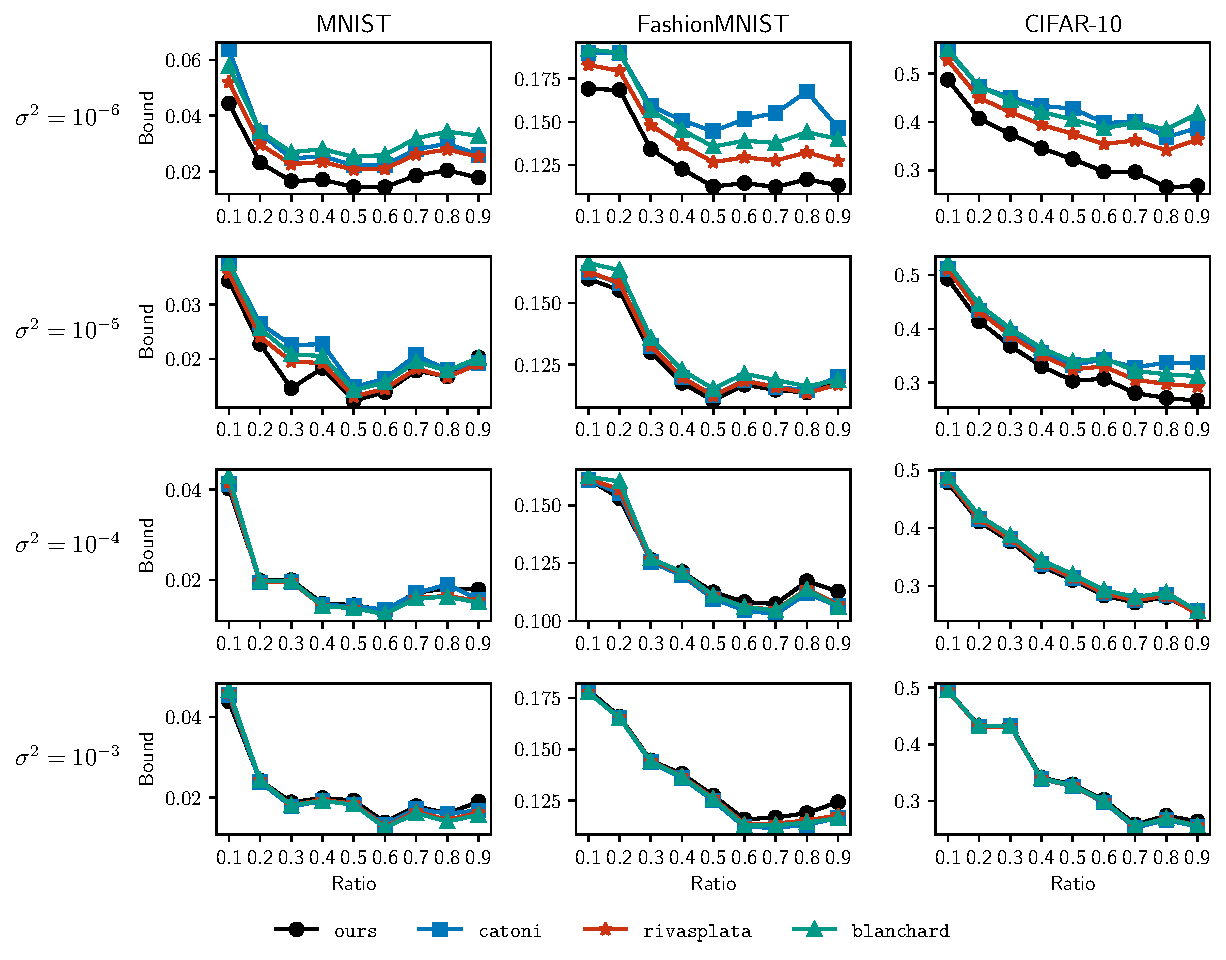
\includegraphics[width=1.0\linewidth]{chapter_6/figures/plot_1_lr_1e-06.pdf}
    \caption[Evolution of the Bound Values in Terms of the Split Ratio (1/2)]{
    Evolution of the bound values in terms of the split ratio. 
    The \mbox{x-axis} represents the different split ratios, and the y-axis represents the bound values obtained after their optimization using our Training Method.
    Each row corresponds to a given variance $\sigma^2$, and each column corresponds to a dataset (MNIST, Fashion-MNIST, or CIFAR-10).
    In this figure, we consider a learning rate of $\lr=10^{-6}$.
    }
    \label{chap:dis-pra:figure:exp-4}
\end{figure}

\begin{figure}
    \centering
    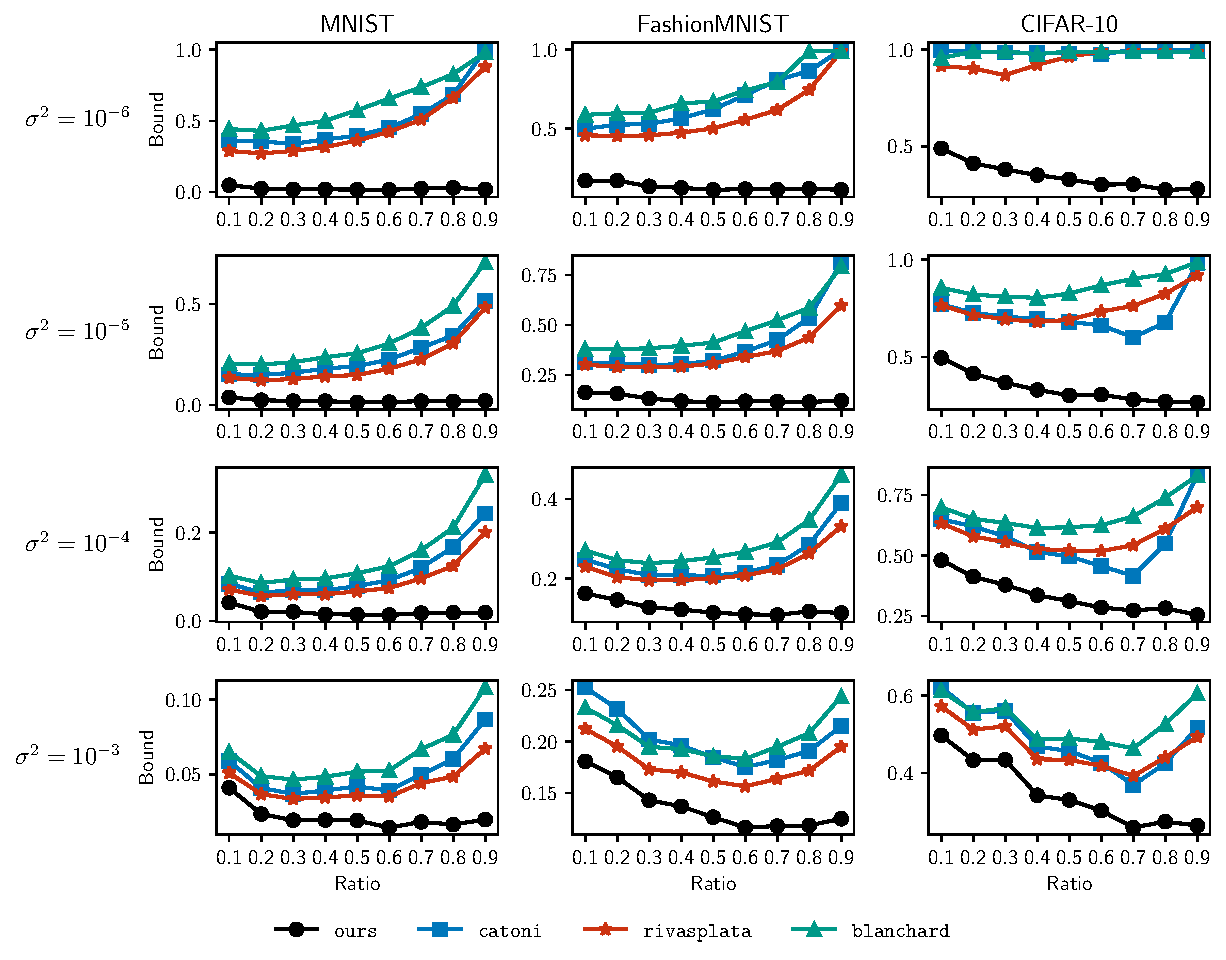
\includegraphics[width=1.0\linewidth]{chapter_6/figures/plot_1_lr_0.0001.pdf}
    \caption[Evolution of the Bound Values in Terms of the Split Ratio (2/2)]{
    Evolution of the bound values in terms of the split ratio. 
    The x-axis represents the different split ratios, and the y-axis represents the bound values obtained after their optimization using our Training Method.
    Each row corresponds to a given variance $\sigma^2$, and each column corresponds to a dataset (MNIST, Fashion-MNIST, or CIFAR-10).
    In this figure, we consider a learning rate of $\lr=10^{-4}$.
    }
    \label{chap:dis-pra:figure:exp-5}
\end{figure}

\subsubsection{Analysis of the Influence of the Split Ratio Between $\S_{\text{prior}}$ and $\S$}

\looseness=-1
\Cref{chap:dis-pra:figure:exp-4,chap:dis-pra:figure:exp-5} study the evolution of the bound values after optimizing the bounds with our Training Method for different parameters.
Specifically, the split ratio of the original train set varies from $0.1$ to $0.9$ ($0.1$ means that $\m_{\text{prior}}= 0.1(\m+\m_{\text{prior}})$), for four variances values $\sigma^2$ and the two learning rates ($\lr=10^{-6}$ and $\lr=10^{-4}$).
For the sake of readability, we present detailed results when the split ratio is $0$ in \Cref{chap:dis-pra:table:1_prior_0.0}.
We first remark that the behavior is different for the two learning rates. 
On the one hand, for $\lr=10^{-6}$, the mean bound values are close to each other, which is not surprising since the disintegrated KL divergences and the \textsc{Rényi} divergences are close to zero (see \Cref{chap:dis-pra:table:1_prior_0.1} to~\Cref{chap:dis-pra:table:1_prior_0.9}). 
Moreover, for MNIST and Fashion-MNIST, there is a trade-off between learning a good prior with $\S_{\text{prior}}$ and minimizing a generalization bound with $\S$.
In this case, the split ratio $0.5$ appears to be a good choice to obtain a tight (disintegrated) PAC-Bayesian bound. 
This ratio is widely used in the PAC-Bayesian literature (see, \eg, in the context of linear classifiers \citep{GermainLacasseLavioletteMarchand2009}, majority votes \citep{ZantedeschiViallardMorvantEmonetHabrardGermainGuedj2021}, and neural networks
\citep{LetarteGermainGuedjLaviolette2019,PerezOrtizRivasplataShaweTaylorSzepesvari2021}).
On the other hand, when $\lr=10^{-4}$, the mean bound values tend to increase when the split ratio increases as well for the bounds introduced in the literature (\ie, for \algoblanchard, \algocatoni, and \algorivasplata), while the mean bound values of our bound remain low.
Indeed, $\m$ decreases as long as the split ratio increases, which has the effect of increasing the bound value drastically when the disintegrated KL divergence is high.
We further explain why the disintegrated KL divergence can become high for the disintegrated bounds of the literature.
To do so, we now restrict our study to a split ratio of $0.5$ in order to {\it (i)} compare the tightness of the bounds, {\it (ii)} understand why the disintegrated bounds of the literature diverge.

\subsubsection{Comparison Between Disintegrated and ``Classic'' Bounds}

We first compare the ``classic'' PAC-Bayesian bound (\Cref{chap:dis-pra:corollary:nn-sto}) and our disintegrated PAC-Bayesian bound (\Cref{chap:dis-pra:corollary:nn}).
To do so, we fix the variance $\sigma^2{=}10^{-3}$ (along with the split ratio equals $0.5$).
We report in \Cref{chap:dis-pra:figure:exp-2}, the mean bound values associated with \algoours (\ie, the Training Method that minimizes our bound) and \algostoNN 
(we recall that \algostoNN is the PAC-Bayesian bound of \Cref{chap:dis-pra:corollary:nn-sto} on the model learned by \algoours).
Actually, \algoours leads to more precise bounds than the randomized \algostoNN even if the two empirical risks are the same and the KL divergence is smaller than the \textsc{Rényi} one.
This imprecision is due to the non-avoidable sampling according to $\Q$ done in the randomized PAC-Bayesian bound of \Cref{chap:dis-pra:corollary:nn-sto} (the \mbox{higher $\K$}, the tighter the bound).
Thus, using a disintegrated PAC-Bayesian bound avoids sampling many NNs to obtain a low risk.
This confirms that our framework makes sense for practical purposes and has a great advantage in terms of time complexity when computing the bounds.

\begin{figure}[!t]
    \centering
    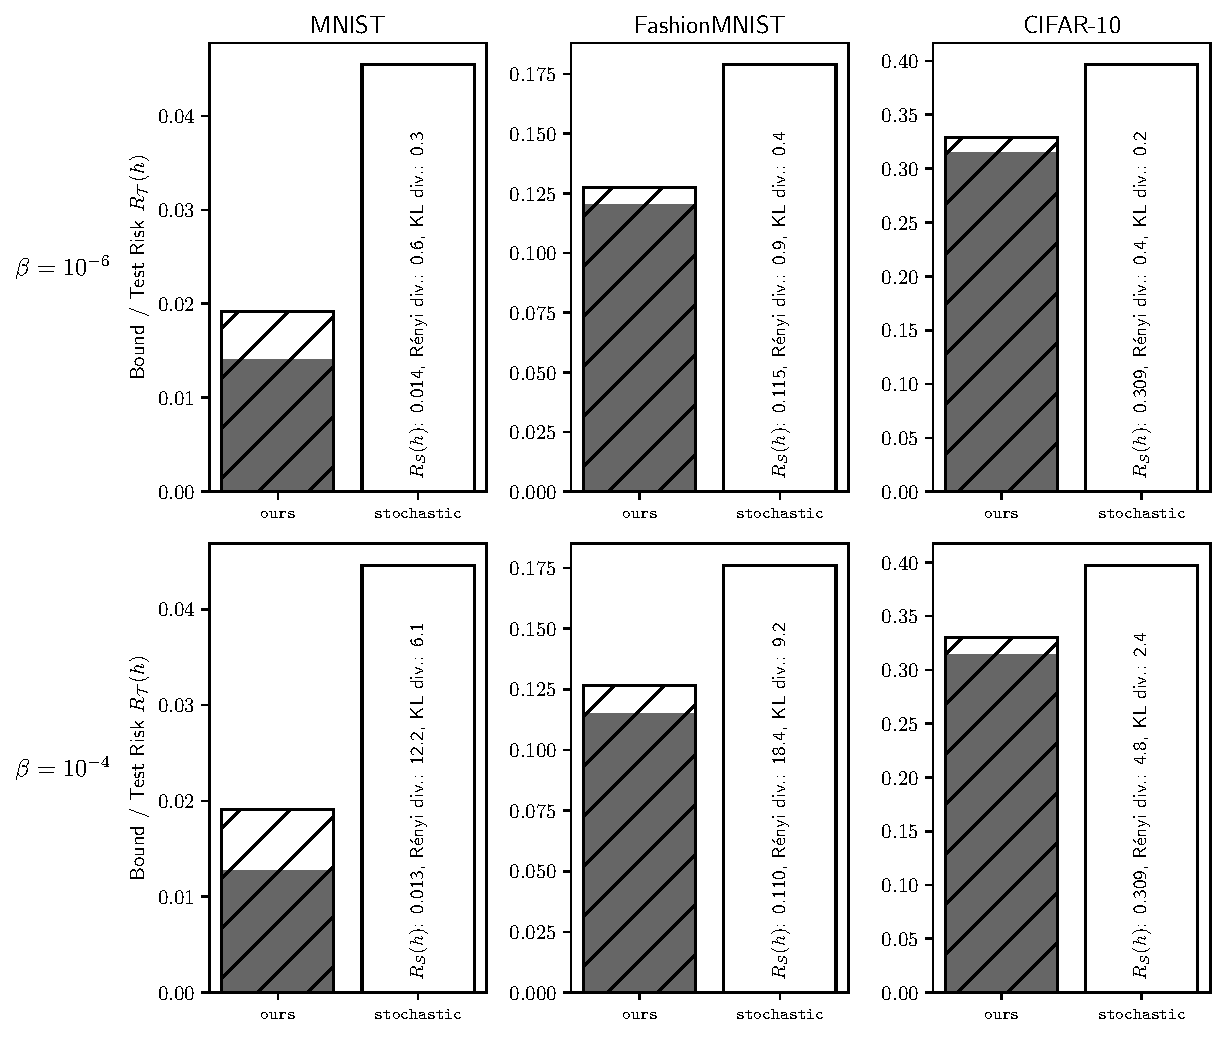
\includegraphics[width=1.0\linewidth]{chapter_6/figures/plot_2_prior_0.5_var_0.001.pdf}
    \caption[Comparisons of the PAC-Bayesian Bounds and the Disintegrated Bounds]{%
    The figure illustrates the values of the PAC-Bayes bound (\Cref{chap:dis-pra:corollary:nn-sto}) and the values of the disintegrated bound (\Cref{chap:dis-pra:corollary:nn}) where the learning rate is $\lr=10^{-4}$ or $\lr=10^{-6}$ and the split ratio is $0.5$.
    The y-axis shows the values of the bounds (the hatched bar for \algoours (\Cref{chap:dis-pra:corollary:nn}) and the white bar for \algostoNN (\Cref{chap:dis-pra:corollary:nn-sto})) and the test risks $\Risk_{\dT}(\h)$ (grey shaded bar).
  We also report the values of the empirical risk $\RiskLoss_{\dS}(\h)$, the \textsc{Rényi} divergence (associated with \algoours' bound), and the KL divergence (associated with \algostoNN's bound). 
}
    \label{chap:dis-pra:figure:exp-2}
\end{figure}

\begin{figure}[!ht]
    \centering
    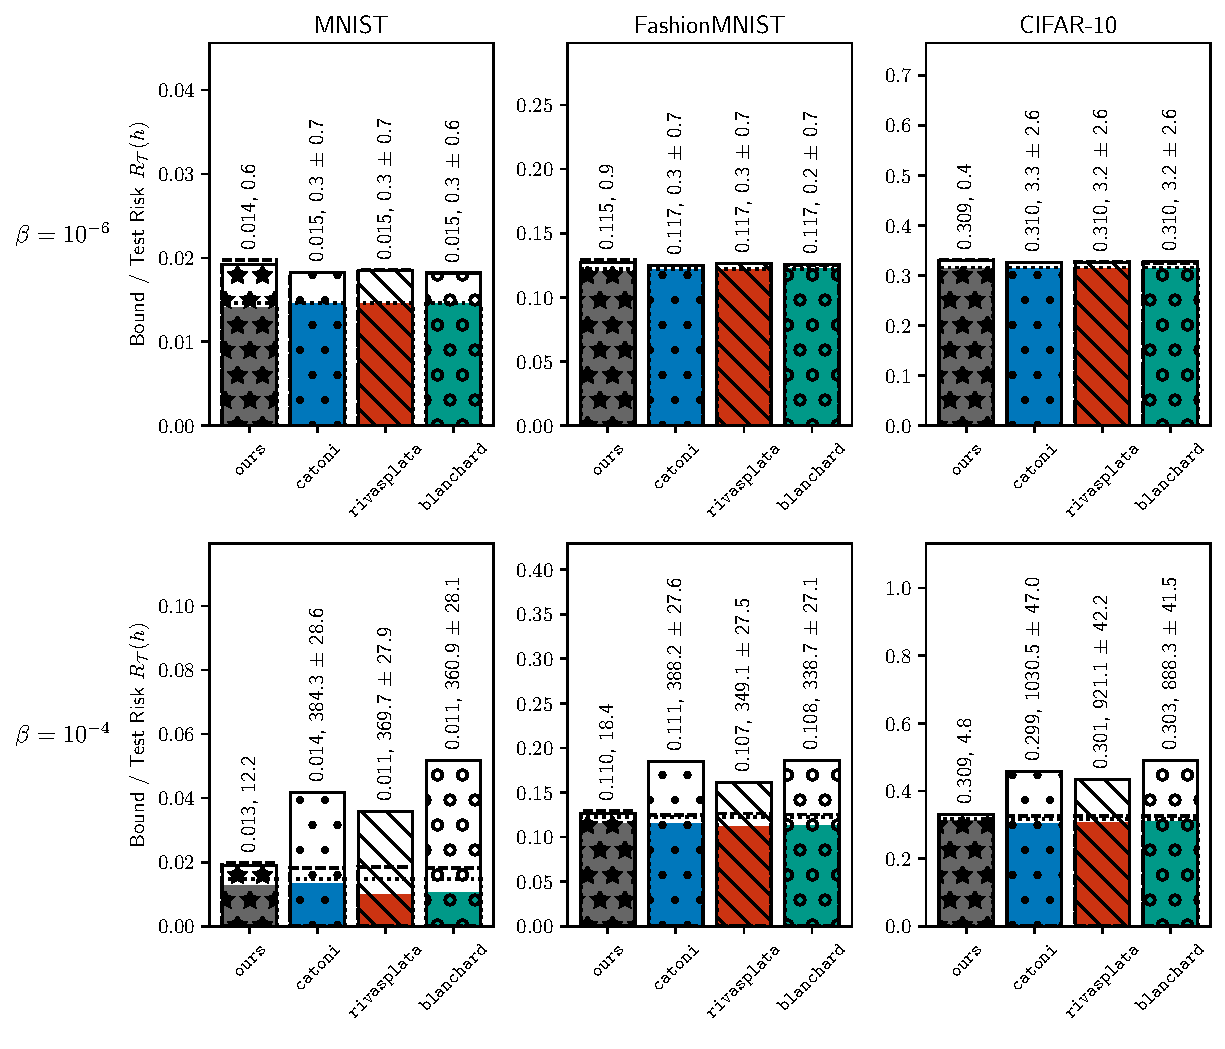
\includegraphics[width=1.0\linewidth]{chapter_6/figures/plot_3_prior_0.5_var_0.001.pdf}
    \caption[Comparison of the Disintegrated Bounds and the Test Risks]{
    This figure shows the value of the disintegrated bounds (the colored bars) and the test risks (the hatched bars) for \Cref{chap:dis-pra:corollary:nn} (``\algoours'') and \Cref{chap:dis-pra:corollary:nn-rbc} (``\algocatoni'', ``\algorivasplata'' and ``\algoblanchard'') in two different settings, \ie, with a learning rate of $\lr=10^{-6}$ and $\lr=10^{-4}$ and with split ratio of $0.5$.
    We also plot the value of the bounds (the dashed lines) and the test risks (the dotted lines) before executing Step {\bf 2)} of our Training Method.
    The y-axis shows the values of the bounds and the test risks $\Risk_{\dT}(\h)$.
    The empirical risk $\Risk_{\dS}(\h)$ is presented above each bar.
    Moreover, the second value represents the mean value of the divergence (the standard deviations are also given for the disintegrated bounds of the literature).
    }
    \label{chap:dis-pra:figure:exp-1}
\end{figure}

\subsubsection{Analysis of  the Tightness of the Disintegrated Bounds}

\looseness=-1
We now compare the tightness of the different disintegrated PAC-Bayesian bounds (\ie, our bound and the ones in the literature). 
We study, as before, the case where the split ratio is $0.5$ and the variance $\sigma^2=10^{-3}$.
We report in \Cref{chap:dis-pra:figure:exp-1} for \algoours, \algorivasplata, \algoblanchard and \algocatoni, the mean bounds values; the mean test risk $\Risk_{\dT}(\h)$ before (\ie, with the prior $\P$) and after applying Step {\bf 2)} (\ie, with the posterior $\AQ$).
Moreover, we report above the bars the mean train risks $\RiskLoss_{\dS}(\h)$ and the mean/standard deviation divergence values obtained after Step {\bf 2)}, \ie, the \textsc{Rényi} divergence $\Renyi_{2}(\AQ\|\P){=}\tfrac{1}{\sigma^2}\|\wbf{-}\vbf_\t\|_{2}^{2}$ for \algoours and the disintegrated KL divergence $\ln\frac{\AQ(\h)}{\P(\h)}{=}\tfrac{1}{2\sigma^2}\left[\| \wbf{+}\epsilonbf{-}\vbf_\t\|^2_{2} {-}\|\epsilonbf\|^2_{2}\right]$ for the others.
First of all, we can remark that we observe two different behaviors for $\lr=10^{-4}$ and $\lr=10^{-6}$. 
For $\lr=10^{-6}$, the bound values are close to each other, as well as the empirical risks and the divergences (which are close to $0$).
In \Cref{chap:dis-pra:figure:exp-1}, we observe that the bound values and the test risks are close to the one associated with the prior distribution because the divergence is close to $0$.
This is probably due to the fact that the learning rate is too small, implying that the bounds are not optimized.
With a higher learning rate of $\lr=10^{-4}$, we observe that our bound remains tight while the disintegrated bounds of the literature are looser.
Hopefully, our bound is improved after performing Step {\bf 2)} of our Training Method.
However, for the bounds of the literature, the value of the disintegrated KL divergence is large, making the bounds looser after executing Step {\bf 2)}.
We now investigate the reasons for the divergence of the bounds
by looking at the influence of the variance $\sigma^2$.

\begin{figure}[t]
    \centering
    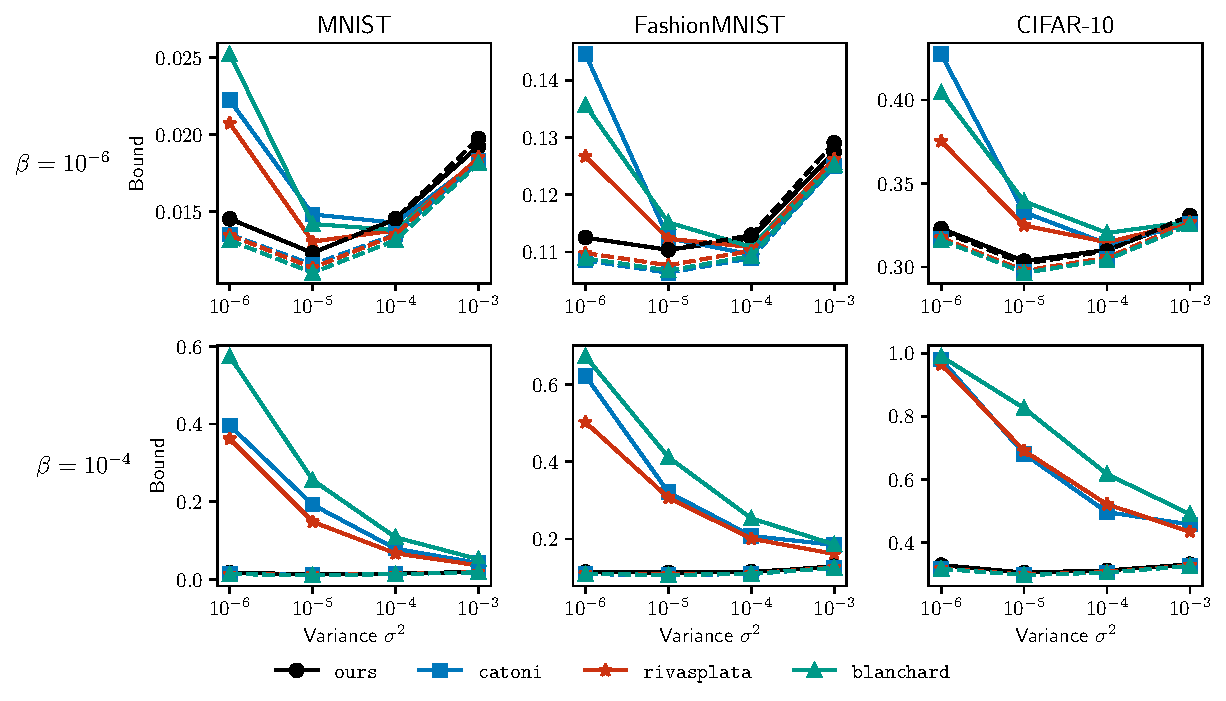
\includegraphics[width=1.0\linewidth]{chapter_6/figures/plot_4_prior_0.5.pdf}
    \caption[Evolution of the Bound Values in Terms of the Variance $\sigma^2$]{
    We plot the evolution of the mean bound values (the plain lines) in terms of the variance $\sigma^2$ after optimizing the bounds with our Training Method.
    Moreover, we plot the mean bound values (the dashed lines) obtained before executing Step {\bf 2)} of our Training Method.
    The variance is represented on the x-axis, while the bound values are represented on the y-axis.  
    Furthermore, each row corresponds to a given learning rate ($\lr=10^{-6}$ or $\lr=10^{-4}$), and each column corresponds to a dataset (either MNIST, FashionMNIST, or CIFAR-10).
    The split ratio considered is $0.5$.
    }
    \label{chap:dis-pra:figure:exp-3}
\end{figure}

\subsubsection{Analysis of the Influence of the Variance $\sigma^2$}

Given a split ratio of $0.5$ and $\lr\in\{10^{-6}, 10^{-4}\}$, we report in \Cref{chap:dis-pra:figure:exp-3} the evolution of the bound values associated with \algoours, \algorivasplata, \algoblanchard, and \algocatoni when the variance varies from $10^{-6}$ to $10^{-3}$.
First of all, an important point is that \algoours behaves differently than \algorivasplata, \algoblanchard, and \algocatoni.
Indeed, for both learning rates, when $\sigma^2$ decreases, the value of our bound remains low, while the others increase drastically due to the explosion of the disintegrated KL divergence term (see \Cref{chap:dis-pra:table:1_prior_0.5} in Appendix for more details).
Concretely, the disintegrated KL divergence in \Cref{chap:dis-pra:corollary:nn-rbc} involves the noise $\epsilonbf$  through  $\frac{1}{2\sigma^2}\| \wbf{+}\epsilonbf{-}\vbf_\t\|_{2}^2{-}\|\epsilonbf\|^2_{2}
$ compared to our divergence which is $\frac{1}{\sigma^2}\| \wbf{-}\vbf_\t\|_{2}^2$ (without noise).
Then, the sampled noise during the optimization procedure $\epsilonbf$ influences the disintegrated KL divergence, making it prone to high variations during training (depending thus on $\sigma^2$).
To illustrate the difference during the optimization, we focus on the objective function (detailed in Appendix) of \Cref{chap:dis-pra:corollary:nn} and \Cref{chap:dis-pra:corollary:nn-rbc} (\Cref{chap:dis-pra:eq:nn-rivasplata}).
Roughly speaking, the divergence in \Cref{chap:dis-pra:corollary:nn} does not depend on the sampled hypothesis $\h$ (with weights $\omegabf+\epsilonbf$), while the divergence of \Cref{chap:dis-pra:eq:nn-rivasplata} does. 
In consequence, the derivatives are less dependent on $\h$ for Corollary~6 than for \Cref{chap:dis-pra:eq:nn-rivasplata}.
To be convinced of this, we propose to study the gradient with respect to the current mean vector $\omegabf$.
On the one hand, the gradient $\frac{\partial \RiskLoss_{\dS}(\h)}{\partial \omegabf}$ of the risk \wrt $\omegabf$ is the same for both bounds (with the loss of \citet{DziugaiteRoy2018}); hence, the phenomenon cannot come from this derivative. 
On the other hand, the gradients of the divergence in  \Cref{chap:dis-pra:eq:nn-rivasplata} and \Cref{chap:dis-pra:corollary:nn} are respectively
\begin{align*}
    \frac{\partial}{\partial \omegabf}\!\!\LB\frac{1}{\m}\!\!\LP\!\frac{\| \omegabf{+}\epsilonbf{-}\vbf_\t\|^2_{2}\!{-}\|\epsilonbf\|^2_{2}}{2\sigma^2}\RP\RB &= \frac{\partial}{\partial \omegabf}\LB \frac{1}{m2\sigma^2}\|\omegabf{+}\epsilonbf{-}\vbf_\t\|_2^2 \RB\\
    &= \frac{1}{m\sigma^2}\LP \omegabf{+}\epsilonbf{-}\vbf_\t\RP = \diamondsuit,\\
    \text{and}\quad\quad  \frac{\partial}{\partial \omegabf}\!\!\LB\frac{1}{\m}\!\!\LP \frac{\|\omegabf{-}\vbf_\t\|_{2}^{2}}{\sigma^2}\RP\RB= &\frac{\partial}{\partial \omegabf}\LB \frac{1}{m\sigma^2}\|\omegabf{-}\vbf_\t\|_2^2 \RB\\
    = &\frac{2}{m\sigma^2}\LP \omegabf{-}\vbf_\t\RP = \heartsuit.
\end{align*}
From the two derivatives, we deduce that $\diamondsuit = \frac{1}{2}\heartsuit + \frac{1}{m\sigma^2}\epsilonbf$.
Hence, each gradient step involves a noise in the gradient of the disintegrated KL divergence \mbox{$\frac{1}{m\sigma^2}\epsilonbf \sim \Ncal({\bf 0}, \frac{1}{\m}\Ibf_D)$}, which is high for a small $\m$.
This randomness causes the disintegrated KL divergence $\frac{1}{2\sigma^2}\| \omegabf{+}\epsilonbf{-}\vbf_\t\|^2_{2}\!{-}\|\epsilonbf\|^2_{2}$ to be larger when $\sigma^2$ decreases since {\it (i)} the divergence is divided by $2m\sigma^2$ and {\it (ii)} the deviation between $\omegabf$ and $\vbf_\t$ increases.
In conclusion, this makes the objective function (\ie, the bound) subjects to high variations during the optimization, implying higher final bound values.
Thus, the \textsc{Rényi} divergence has a valuable asset over the disintegrated KL divergence since it does not depend on the sampled noise $\epsilonbf$.

\subsubsection{Take Home Message from the Experiments}
To summarize, our experiments show that our disintegrated bound is, in practice, tighter than the ones in the literature.
This tightness allows us to precisely bound the true risk $\Risk_{\D}(\h)$ (or the test risk $\Risk_{\dT}(\h)$); thus, the model selection from the disintegrated bound is effective.
Moreover, we show that our bound is more easily optimizable than the others. 
This is mainly due to the disintegrated KL divergence, which depends on the sampled hypothesis $\h$ with weights $\omegabf{+}\epsilonbf$.
Indeed, the gradients of the disintegrated KL divergence with respect to $\omegabf$ include the noise $\epsilonbf$, making the gradient inaccurate (especially with a ``high'' learning rate and small variance $\sigma^2$).

\section{Perspectives for the Majority Vote}

Before concluding, we discuss some perspectives for the stochastic majority vote introduced in \Cref{chap:mv-sto}.
Recall that the {\it stochastic} majority vote has its weights $\Q$ sampled from the Dirichlet distribution $\hyperQ$ defined as $\hyperQ(\Q) \triangleq \frac{1}{Z(\paramDir)}\prod_{j=1}^{\card(\H)}\Q(\h_j)^{\sparamDir_j-1}$ (also called hyper-posterior).
One drawback of the PAC-Bayesian approach for the {\it stochastic} majority vote in \Cref{chap:mv-sto} is that we are not considering only one majority vote (with weights sampled from the hyper-posterior $\hyperQ$).
Moreover, based on the margin theory~\citep[initiated by][]{SchapireFreundBarlettLee1998} and our work in \Cref{chap:mv-sto}, \citet{BiggsZantedeschiGuedj2022} derived PAC-Bayesian bound for the expected majority vote.
This latter work illustrates that a special care is unfortunately needed to obtain a bound for a unique majority vote through the PAC-Bayesian theory.
Hopefully, thanks to the disintegrated PAC-Bayesian framework, we can bound the true risk of a single majority vote classifier.
As an illustration we derive two bounds for such a classifier based on \citet{RivasplataKuzborskijSzepesvariShaweTaylor2020}'s bound (\Cref{chap:pac-bayes:theorem:general-disintegrated-rivasplata}) and based on \Cref{chap:dis-pra:theorem:disintegrated}.

\begin{restatable}[Instantiation of \Cref{chap:pac-bayes:theorem:general-disintegrated-rivasplata} to Stochastic Majority Votes]{corollary}{corollarydisintegratedrivmv}\label{chap:dis-pra:corollary:disintegrated-riv-mv}
For any distribution $\D$ on $\X{\times}\Y$, for any finite set of voters $\H$, for any hyper-prior distribution $\hyperP=\Dir(\paramDirP)$ on $\H$ with $\paramDirP\in(\Rbb^{+}_{*})^{\card(\H)}$, for any loss $\loss: \H\times(\X{\times}\Y)\to [0,1]$, for any $\delta \in (0, 1]$, for any algorithm \mbox{$A$} that outputs a hyper-posterior given a learning sample and a hyper-prior, with probability at least $1{-}\delta$ over the learning sample $\S{\sim}\D^{\m}$ and the posterior distribution $\Q{\sim} \hyperAQ=\Dir(\paramDir)$ with $\paramDir\in(\Rbb^{+}_{*})^{\card(\H)}$ we have
\begin{align*}
    \kl(\RiskLoss_{\dS}(\MVQ)\|\RiskLoss_{\D}(\MVQ)) \le \frac{1}{\m}\!\LB\ln\frac{Z(\paramDirP)}{Z(\paramDir)} + \!\!\!\!\sum_{j=1}^{\card(\H)}\!\!(\sparamDir_j-\sparamDirP_j)\ln(\Q(\h_j)) + \ln\frac{2\sqrt{\m}}{\delta}\RB,
\end{align*}
\mbox{where $\hyperAQ{\defeq}A(\S,\hyperP)$ is output by the deterministic algorithm $A$}.
\end{restatable}
\begin{noaddcontents}\begin{proof}
Deferred to~\Cref{ap:dis-pra:sec:proof-disintegrated-riv-mv}
\end{proof}\end{noaddcontents}


\begin{restatable}[Instantiation of \Cref{chap:dis-pra:theorem:disintegrated} to Stochastic Majority Votes]{corollary}{corollarydisintegratedmv}\label{chap:dis-pra:corollary:disintegrated-mv}
For any distribution $\D$ on $\X{\times}\Y$, for any finite set of voters $\H$, for any hyper-prior distribution $\hyperP=\Dir(\paramDirP)$ on $\H$ with $\paramDirP\in(\Rbb^{+}_{*})^{\card(\H)}$, for any loss $\loss: \H\times(\X{\times}\Y)\to [0,1]$, for any $\lambda>1$, for any $\delta \in (0, 1]$, for any algorithm \mbox{$A$} that outputs a hyper-posterior given a learning sample and a hyper-prior, with probability at least $1{-}\delta$ over the learning sample $\S{\sim}\D^{\m}$ and the posterior distribution $\Q{\sim} \hyperAQ=\Dir(\paramDir)$ with $\paramDir\in(\Rbb^{+}_{*})^{\card(\H)}$ we have
\begin{align*}
    \kl(\RiskLoss_{\dS}(\MVQ)\|\RiskLoss_{\D}(\MVQ)) \le \frac{1}{\m}\Bigg[&{\frac{2\lambda{-}1}{\lambda{-}1}}\ln\frac{2}{\delta}+ \ln\frac{Z(\paramDirP)}{Z(\paramDir)}\\
    &+ \frac{1}{\lambda{-}1}\ln\frac{Z(\lambda\paramDir{+}(1{-}\lambda)\paramDirP)}{Z(\paramDir)} + \ln(2\sqrt{m})\Bigg],
\end{align*}
\mbox{where $\hyperAQ{\defeq}A(\S,\hyperP)$ is output by the deterministic algorithm $A$}.
\end{restatable}
\begin{noaddcontents}\begin{proof}
Deferred to~\Cref{ap:dis-pra:sec:proof-disintegrated-mv}
\end{proof}\end{noaddcontents}

These two bounds offer great perspectives to upper-bound the true risk of the majority vote.
First, as we can remark, the two theorems holds for all (bounded) losses $\loss()$ including the 01-loss.
Hence, the true risk $\Risk_{\D}(\MVQ)$ can be upper-bounded directly without using the $\frac{1}{2}$-margin of \citet{LavioletteMorvantRalaivolaRoy2017} as in \Cref{chap:mv-sto}.
While our bounds require to sample a single majority vote from $\hyperQ$, they might be tighter since it does not rely on margin bound \citep[as][]{BiggsZantedeschiGuedj2022} and directly deal with the 01-loss.


\section{Summary and Conclusion}
\label{chap:dis-pra:sec:conclu}

We provide a new and general disintegrated PAC-Bayesian bound (\Cref{chap:dis-pra:theorem:disintegrated}) in the family of disintegrated PAC-Bayesian bounds (\Cref{chap:pac-bayes:def:disintegrated-pac-bayes}), \ie, when the derandomization step consists in {\it (i)} learning a posterior distribution $\AQ$ on the classifiers set (given an algorithm, a learning sample $\S$ and a prior distribution $\P$) and {\it (ii)} sampling a hypothesis $\h$ from this posterior $\AQ$.
While our bound can be looser than the ones of \citet{RivasplataKuzborskijSzepesvariShaweTaylor2020,BlanchardFleuret2007,Catoni2007}, it provides nice opportunities for learning deterministic classifiers.
Indeed, our bound can be used not only to study the theoretical guarantees of deterministic classifiers but also to derive self-bounding algorithms (based on the bound optimization) that are more stable and efficient than the ones we obtain from the bounds of the literature.
Concretely, the bounds of \citet{RivasplataKuzborskijSzepesvariShaweTaylor2020,BlanchardFleuret2007,Catoni2007} depend on two terms related to the classifier drawn: the risk and the ``disintegrated KL divergence'', while in our bound the (\textsc{Rényi}) divergence term depends on the hypothesis set, implying that the divergence remains the same whatever which classifier is drawn.  
In this sense, our bound is more stable as the learning algorithm seeking to minimize the bound allows, in practice, to choose a better hypothesis than with the bounds of \citet{RivasplataKuzborskijSzepesvariShaweTaylor2020,BlanchardFleuret2007,Catoni2007}.
We have illustrated the interest of our bound on neural networks and provides perspectives on the the stochastic majority vote classifier introduced in \Cref{chap:mv-sto}.\\

One future research direction related to this work is to develop new proof techniques to convert generalization bounds holding in expectation \citep[see \eg,][]{XuRaginsky2017} to high-probability bounds.
To do so, one can apply \textsc{Markov}'s Inequality (\Cref{ap:tools:theorem:first-markov}) and the \textsc{Donsker}-\textsc{Varadhan} Variational Representation of the KL divergence to obtain a high-probability bound with the bound in expectation as upper-bound.
This work might be significant since the dependence in $\delta$ is, for now, only polynomial, while a logarithmic dependence is preferable.
However, the limitation would be that the bound in expectation must consider a specific distribution (related to the \textsc{Donsker}-\textsc{Varadhan} Variational Representation).\\

In the next chapter, we leverage the disintegrated KL divergence and the bound of \citet{RivasplataKuzborskijSzepesvariShaweTaylor2020} to obtain generalization bounds with an arbitrary complexity measure.
Hence, given a complexity measure defined by the user, we are able to give a generalization bound that holds with high probability over the learning sample and a hypothesis sampled from a complexity-measure-dependent distribution.
Moreover, the bound with arbitrary complexity measures encompasses the generalization bounds of the literature and is recalled in \Cref{chap:intro}.